\begin{figure}[h]
\centering
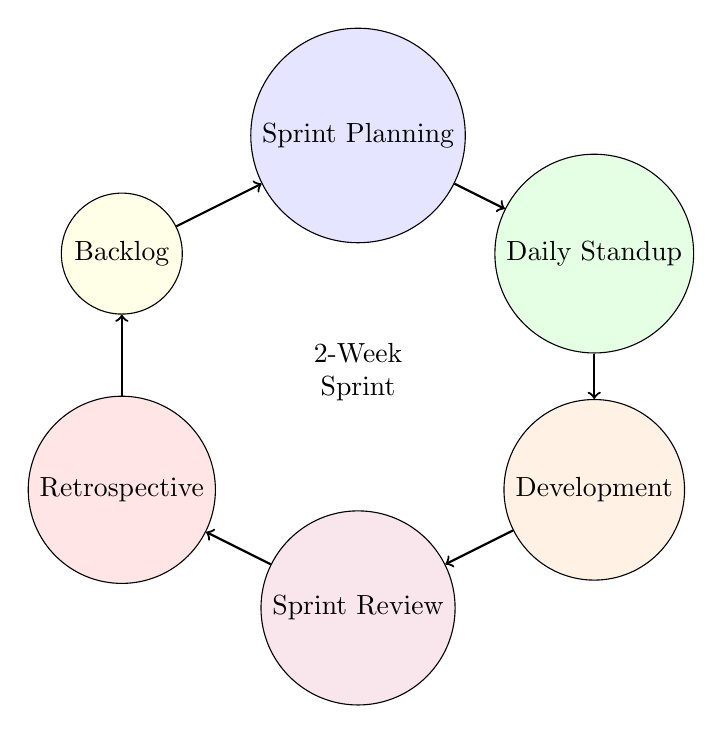
\begin{tikzpicture}
    % Sprint cycle circle
    \node[draw, circle, fill=blue!10, minimum size=1.5cm] (planning) at (0,3) {Sprint Planning};
    \node[draw, circle, fill=green!10, minimum size=1.5cm] (daily) at (3,1.5) {Daily Standup};
    \node[draw, circle, fill=orange!10, minimum size=1.5cm] (development) at (3,-1.5) {Development};
    \node[draw, circle, fill=purple!10, minimum size=1.5cm] (review) at (0,-3) {Sprint Review};
    \node[draw, circle, fill=red!10, minimum size=1.5cm] (retro) at (-3,-1.5) {Retrospective};
    \node[draw, circle, fill=yellow!10, minimum size=1.5cm] (backlog) at (-3,1.5) {Backlog};

    % Arrows showing cycle
    \draw[->, thick] (planning) -- (daily);
    \draw[->, thick] (daily) -- (development);
    \draw[->, thick] (development) -- (review);
    \draw[->, thick] (review) -- (retro);
    \draw[->, thick] (retro) -- (backlog);
    \draw[->, thick] (backlog) -- (planning);

    % Center label
    \node[align=center] at (0,0) {2-Week\\Sprint};

\end{tikzpicture}
\caption{Sprint Cycle: Ahmed's team follows a two-week sprint cadence with regular ceremonies for planning, coordination, review, and continuous improvement.}
\label{fig:sprint-cycle}
\end{figure}
